\chapter{Bayesian estimation } \label{chap:estimation}

The practical use the GLLAMM developed in chapter \ref{chap:framework} requires the estimation of all of the items and individuals' dimensions, loadings, regression and structural parameters. These can be obtained within two frameworks: the frequentist and bayesian. 

The current chapter center its attention on describing the bayesian estimation procedure, using the Markov Chain Monte Carlo method (MCMC). For a full development of GLLAMM under the frequentist framework refer to Rabe-Hesketh and colleagues \cite{Rabe_et_al_2004a, Rabe_et_al_2004b, Skrondal_et_al_2004a, Rabe_et_al_2012}.

%%%%%%%%%%%%%%%%%%%%%%%%%%%%%%%%%%%%%%%%%%%%%%%%%%%%%%%%%%%%%%%%%%%%%%%
%%%%%%%%%%%%%%%%%%%%%%%%%%%%%%%%%%%%%%%%%%%%%%%%%%%%%%%%%%%%%%%%%%%%%%%

\section{Benefits and shortcomings}

\subsection{Why Bayesian?} \label{sub_sect:goods}

The reasons on why bayesian statistics is attractive to perform the parameters' estimation of any model, and especially for the GLLAMM developed in chapter \ref{chap:framework}, are:

\begin{enumerate}	
	\item It is built on a simulation-based estimation method, therefore, it can handle all kinds of priors and data-generating processes \cite{Fox_2010}. This is especially useful with highly complex and over-parameterized models, where other methods are unfeasible or work poorly \cite{Baker_1998, Kim_1999}. 
	
	\item While the likelihood functions are used to define the posterior sampling distributions, they can also be used in a generative way. The likelihood for the data, and priors for the parameters, form the basis to produce samples from the posterior distribution. However, they can also be used to simulate observations, allowing us to test the ability of the method/data to recover the parameters of interest \cite{McElreath_2020}.
	
	\item The bayesian estimates are at least as good as its frequentist counterparts \cite{Baker_1998, Wollack_2002, Hsieh_2010}. This is true when the method uses uninformative `flat' priors. However, because the procedure allow us to integrate prior knowledge about the parameters, beyond the observed responses, it can produce results even in scenarios where the Maximum Likelihood methods (ML) have issues of non-convergence or improper estimation \cite{Skrondal_et_al_2004a, Fox_2010, McElreath_2020}. Examples of such are: 
	
	\begin{enumerate}
		\item when we have small sample sizes.
		
		\item when individuals have null scores or aberrant response patterns \cite{Hambleton_et_al_1991a, Azevedo_2003}. The latter happens when examinees answer some relatively difficult and discriminating items correctly, while answering some of the easiest incorrectly.
		
		\item when parameters need to be confined to a permitted space, e.g. the estimation of positive unique factors variances \cite{Martin_et_al_1975}.
		
		\item when we need to estimate parameters under sparse data, where the asymptotic theory is unlikely to hold \cite{Fox_2010};
		
	\end{enumerate}
	
\end{enumerate}

%%%%%%%%%%%%%%%%%%%%%%%%%%%%%%%%%%%%%%%%%%%%%%%%%%%%%%%%%%%%%%%%%%%%%%%

\subsection{Are you sure there's nothing wrong?} \label{sub_sect:bads}
Off course the bayesian framework has shortcomings, among them:

\begin{enumerate}	
	\item It exposes the user to somewhat-arbitrary decisions about the running of the chains, in order to ensure a proper performance, e.g. how many iterates does the chain need to achieve precise estimates?, what is the right size for the burn-in and warm-up phases?, how should the thinning procedure be performed, if any?, should we follow the same procedure for all parameters of interest?, among others \cite{Skrondal_et_al_2004a}. 
	
	\item The user can include all type of information through the priors distributions, making their elicitation convenient for manipulation.
	
	\item Multiple options are available to evaluate the performance of the method, and most of them are visual, making it hard to assess if a proper posterior investigation have been made \cite{Gelman_et_al_1996a}. More specifically, the user has multiple options to assess if the chain achieves the three requirements of a good performance: stationarity, convergence, and good mixing \cite{McElreath_2020}. 
	
	\item The procedure makes it hard to discover parameters' lack of identification \cite{Skrondal_et_al_2004a}. Inadequate mixing of the chain could lead us to think unidentified parameters have been estimated with precision, when in fact what we have are `flat' posteriors \cite{Keane_1992}.
	
	\item Oftentimes the posterior sampling geometry of the model makes it hard to find proper solutions for the parameter space, no matter the rotation/rescaling of the parameter, or the amount of data \cite{Betancourt_et_al_2013}. This is especially true in complex hierarchical models.
	
	\item The greater the complexity of the model, the harder it is to communicate/share the implementation with other scientist. This is especially true, when researcher re-parameterize the model to solve the previous shortcoming \cite{McElreath_2020}.
	
	\item The procedure usually requires more time to achieve a proper solution, compared to the classical methods. This is especially true in models with high complexity \cite{Tarazona_2013, Rivera_2019}.
\end{enumerate}

Although some of the previous shortcomings have made the Bayesian procedure a ``controversial" implementation, most of them already have acceptable solutions. 

For the first point, a popular approach is to use a large number of iterates, burn-in and thinning processes. This is mostly applicable under the Metropolis-Hastings and Gibbs sampling algorithms. However, recent solutions, like the Hamiltonian Monte Carlo (HMC) \cite{Betancourt_et_al_2013}, is less reliant on selecting these features, as it implements a different sampling mechanism (see section \ref{sub_sect:hmc}). 

On the second point, the literature has indicated that priors can be used to reflect subjective beliefs\footnote{see \citet{McElreath_2020} (Chapter 2, pp. 36), Rethinking section ``Prior, prior pants on fire", for an interesting stance contrary to this statement.}. However, as \citet{McElreath_2020} indicated, because the priors can be considered a part of the model assumptions, they can be chosen, evaluated, and revised as any other component of the model, through the use of prior predictive simulations and/or sensitivity analysis  (see section \ref{sub_sect:prior_pred}).

About the third point, the literature on bayesian analysis acknowledge that the visual assessment of stationarity and convergence is easier, and these procedures usually has additional support from statistics like \texttt{Rhat} \cite{Gelman_et_al_2014}. On the contrary, a visual evaluation of `good' mixing remains as a hard task. Recent approaches have taken a more proactive stance on the latter, seeking to increase the possibility of a well mixed chain by changing the posterior sampling geometry of the model \cite{Papaspiliopoulos_et_al_2003, Papaspiliopoulos_et_al_2007, Betancourt_et_al_2013, McElreath_2020} (see section \ref{sect:noncenter}).

On the fourth point, the most common solution is to use regularizing priors, i.e. priors that are more `skeptical' of wider parameter spaces \cite{McElreath_2020}. However, it is important to mention, there are scenarios where one achieves poor parameter estimates, even in the presence of `enough' data and regularizing priors, but this shortcoming is also applicable to the classical estimation procedures, e.g. the estimation of the variance parameters in random effects models \cite{Skrondal_et_al_2004a}.

About the fifth point, as it was mentioned in previous paragraphs, a recent approach to solve the issue is to change the posterior sampling geometry of the model. This means to re-parameterize the model in a way that removes the dependence of the parameters on other sampled parameters; or even, produce sample mechanisms located in a continuous between a centered (CP) and non-centered parametrization (NCP), e.g. Interleaved HMC (iHMC) and/or Variational Inference (VI) \cite{Gelfand_et_al_1995, Gelfand_et_al_1996, Papaspiliopoulos_et_al_2003, Papaspiliopoulos_et_al_2007, Betancourt_et_al_2013, Gorinova_et_al_2019} (see section \ref{sect:noncenter}).

Finally, the sixth and seventh points can be considered the `price' a scientist has to pay, to be able to fit models that conforms better with the observed data generating processes. Although, recent developments are striving to improve upon reducing the latter, i.e. the required running time.

%%%%%%%%%%%%%%%%%%%%%%%%%%%%%%%%%%%%%%%%%%%%%%%%%%%%%%%%%%%%%%%%%%%%%%%
%%%%%%%%%%%%%%%%%%%%%%%%%%%%%%%%%%%%%%%%%%%%%%%%%%%%%%%%%%%%%%%%%%%%%%%

\section{Bayesian GLLAMM for dichotomous outcomes} \label{sect:model}

\subsection{Posterior distribution}

Denoting $\mathbf{Y}$ as the observed data and $\pmb{\Omega} = \{ \pmb{\beta}, \pmb{\Lambda}, \pmb{\Theta}, \pmb{\Psi}, \pmb{\Gamma} \}$, i.e. all the parameters declared in section \ref{s_sect:response} and \ref{s_sect:struct}, the posterior distribution is obtained using the Bayes theorem, in the following way:
%
\begin{equation} \label{eq:posterior1}
	\begin{split}
		P(\pmb{\Omega} \; | \; \mathbf{Y}) = \frac{ P( \mathbf{Y} \; | \; \pmb{\Omega} ) \; P( \pmb{\Omega} ) }{ \int P( \mathbf{Y} \; | \; \pmb{\Omega} ) \; P( \pmb{\Omega} ) \; d\pmb{\Omega} } \\
	\end{split}
\end{equation}

\noindent this is possible since the Bayesian approach makes no distinction between latent variables and parameters. All of them are considered random quantities \cite{Skrondal_et_al_2004a}. Furthermore, since inference only requires representing the likelihood of the data $P( \mathbf{Y} \; | \; \pmb{\Omega} )$ and the prior distribution $P( \pmb{\Omega} )$; and because the denominator is just a (hard to calculate) constant, the posterior can be determined up to a normalizing constant, without loss of generality:
%
\begin{equation} \label{eq:posterior2}
	\begin{split}
		P(\pmb{\Omega} \; | \; \mathbf{Y}) &\propto P( \mathbf{Y} \; | \; \pmb{\Omega} ) \; P( \pmb{\Omega} )
	\end{split}
\end{equation}

%%%%%%%%%%%%%%%%%%%%%%%%%%%%%%%%%%%%%%%%%%%%%%%%%%%%%%%%%%%%%%%%%%%%%%%

\subsection{Prior distributions} \label{sub_sect:priors}

Similar to \citet{Patz_et_al_1999}, we use an independent distributional structure for the joint priors of the parameters. Therefore, at the highest level of the GLLAMM we have:
%
\begin{equation} \label{eq:priors}
	\begin{split}
		P( \pmb{\Omega} ) & = P( \pmb{\beta}, \pmb{\Lambda}, \pmb{\Theta}, \pmb{\Psi}, \pmb{\Gamma} ) \\
		%
		&= P( \pmb{\beta} ) \; P( \pmb{\Lambda} ) \; P( \pmb{\Theta} ) \; P( \pmb{\Psi} ) \; P( \pmb{\Gamma} ) \\
		%	
		&= P( \pmb{\beta} ) \; \left[ P( \pmb{\alpha} ) \; P( \pmb{\lambda} ) \right] \; \left[ P( \pmb{\eta} ) \; P( \pmb{\theta} ) \right] \; \left[ P( \pmb{\Psi}_{\eta} ) \; P( \pmb{\Psi}_{\theta} ) \right] \; \left[ P( \pmb{\Gamma}_{\eta} ) \; P( \pmb{\Gamma}_{\theta} ) \right]
	\end{split}
\end{equation}

However, giving the hierarchical and cross-classified structure of the model, the lower level priors will also depend on further parameters\footnote{Because of this sequential model specification, it is said the priors also have a ``hierarchical" structure.}, e.g. variances and covariances of the latent variables. These are known as \textit{hyper-parameters}, and their prior distributions as \textit{hyper-priors}. Because of the previous, we are not going to detail their lower level representation, as they are highly dependent on the specifics of the model.

Section \ref{sub_sect:prior_pred} details the process of prior predictive investigation for prior elicitation. On the other hand, chapter \ref{chap:simulation} and \ref{chap:application} will show the elicitation of priors, in the context of a simulated and real data set, respectively.

%%%%%%%%%%%%%%%%%%%%%%%%%%%%%%%%%%%%%%%%%%%%%%%%%%%%%%%%%%%%%%%%%%%%%%%

\subsection{Likelihood}

Following \citet{Rabe_et_al_2004a}, the likelihood function is build in a recursive way. 

\noindent First, we replace the structural model (\ref{eq:structural_model1}) into the linear predictor (\ref{eq:linear_predictor3}):
%
\begin{equation} \label{eq:lin_pred}
	\begin{split}
		v_{jkd} &= \mathbf{X}_{j} \pmb{\beta} + ( \mathbf{I} - \pmb{\Psi} )^{-1} \left[ \pmb{\Gamma} \mathbf{W} + \pmb{\zeta} \right] \; \pmb{\Lambda} \; \mathbf{H}_{j}
	\end{split}
\end{equation}

\noindent Second, the linear predictor and inverse-link function (\ref{eq:response_dich1}) are used to construct the systematic part of the response (\ref{eq:systematic}), i.e. its expected value. Here we use a logit link for pedagogical purposes:
%
\begin{equation} \label{eq:prob}
	\begin{split}
		\pi_{jkd} &= \frac{ \text{exp}(\tau_{k} + v_{jkd}) }{ 1 + \text{exp}(\tau_{k} + v_{jkd}) } = \frac{ \text{exp}(v_{jkd}) }{ 1 + \text{exp}(v_{jkd}) }
	\end{split}	
\end{equation}

\noindent Third, the expected value is used in the distributional part (\ref{eq:distributional}), in the following form:
%
\begin{equation} \label{eq:dist}
	\begin{split}
		f \left( y_{jkd}=1 \; | \; \mathbf{X}, \mathbf{W}, \pmb{\Omega} \right) &= \pi_{jkd}^{n} (1 - \pi_{jkd})^{1-n}
	\end{split}
\end{equation}

\noindent Fourth, considering assumptions (M1) and (M2) described in section \ref{s_sect:assump}, we produce the level-1 likelihood:
%
\begin{equation} \label{eq:lik1}
	f \left( \mathbf{y}=\mathbf{1} \; | \; \mathbf{X}, \mathbf{W}, \pmb{\Omega} \right) = \prod_{j=1}^{J} \prod_{d=1}^{D} \prod_{k=1}^{K} f \left( y_{jkd}=1 \; | \; \mathbf{X}, \mathbf{W}, \pmb{\Omega} \right)
\end{equation}

\noindent Fifth, we define the marginal likelihood at levels $l$ and $m$, conditional on the latent variables at levels $l+1$ and $m+1$, in the following form:
%
\begin{equation} \label{eq:lik2}
	f^{(l)}_{(m)} \left( \mathbf{y}=\mathbf{1} \; | \; \mathbf{X}, \mathbf{W}, \pmb{\Omega} \right) = \int \left[ \prod f^{(l-1)}_{(m-1)} \left( \mathbf{y}=\mathbf{1} \; | \; \mathbf{X}, \mathbf{W}, \pmb{\Omega} \right) \right] \; P( \pmb{\Theta}^{(l)}_{(m)} ) \; d\pmb{\Theta}^{(l)}_{(m)}
\end{equation}

\noindent where the product inside the brackets is over all units in level $(l-1)$ and $(m-1)$, the first level is defined as in equation (\ref{eq:lik1}), and $P( \pmb{\Theta}^{(l)}_{(m)} )$ are the prior distributions for the latent variables at level $l$ and $m$, with $\pmb{\Theta}^{(l)}_{(m)} = [\pmb{\eta}^{(m)}, \pmb{\theta}^{(l)}]$. Finally, we define the likelihood as:
%
\begin{equation} \label{eq:lik3}
	\mathcal{L}(\mathbf{X}, \mathbf{W}, \pmb{\Omega}) = \prod_{m=2}^{M+1} \prod_{l=2}^{L+1} f^{(l)}_{(m)} \left( \mathbf{y}=\mathbf{1} \; | \; \mathbf{X}, \mathbf{W}, \pmb{\Omega} \right)
\end{equation}

\noindent and the log-likelihood as:
%
\begin{equation} \label{eq:loglik}
	\ell(\mathbf{X}, \mathbf{W}, \pmb{\Omega}) = \log \mathcal{L}(\mathbf{X}, \mathbf{W}, \pmb{\Omega})
\end{equation}

%%%%%%%%%%%%%%%%%%%%%%%%%%%%%%%%%%%%%%%%%%%%%%%%%%%%%%%%%%%%%%%%%%%%%%%
%%%%%%%%%%%%%%%%%%%%%%%%%%%%%%%%%%%%%%%%%%%%%%%%%%%%%%%%%%%%%%%%%%%%%%%

\subsection{Model identification} \label{sect:identification}

As indicated by \citet{Rabe_et_al_2004a}, in order to fully specify the model and provide a scale for the latent variables, we have to make assumptions for either the distribution of the disturbances $\pmb{\zeta}$, or the distribution of one or more of the latent variables $\pmb{\Theta}$. On the other hand, as point out by \citet{Fujimoto_2018b} and several others authors, we could also set restrictions for one or more of the loadings in $\pmb{\Lambda}$. The last is more prevalent in frequentist software packages like Winsteps \cite{Winsteps2021}.

Furthermore, as it is hinted by equation (\ref{eq:lik3}), it is assumed the latent variables at different levels are independent from each other, whereas latent variables at the same level may present dependency. Therefore, when the assumption is coherent under the context of a model, we will presume the latent variables at the same level have a multivariate normal distribution with a mean and covariance structure determined by equations (\ref{eq:structural_model2}) and (\ref{eq:structural_model3}). In the case of the covariance matrices, these are determined by the covariance of the specific disturbances $\pmb{\zeta}$. 

Chapter \ref{chap:simulation} and \ref{chap:application} will show the model identification strategy in the context of a simulated and real data set, respectively.

%%%%%%%%%%%%%%%%%%%%%%%%%%%%%%%%%%%%%%%%%%%%%%%%%%%%%%%%%%%%%%%%%%%%%%%
%%%%%%%%%%%%%%%%%%%%%%%%%%%%%%%%%%%%%%%%%%%%%%%%%%%%%%%%%%%%%%%%%%%%%%%


\section{Computational implementation} \label{sect:comp_imp}

\subsection{Hamiltonian Monte Carlo} \label{sub_sect:hmc}

For years the state-of-the-art platform for Bayesian statistical modeling have been the BUGS\footnote{Bayesian inference Using Gibbs Sampling} project, with its WinBUGS and OpenBUGS implementations \cite{Lunn_et_al_2000, Lunn_et_al_2009}. However, a more recent participant JAGS\footnote{Just Another Gibbs Sampling} \cite{Plummer_2003} has gain traction, due to its cross-platform capabilities. In any case, both platforms are not that different form each other. Both use two of the most popular and successful algorithms for performing MCMC: the Metropolis-Hastings \cite{Metropolis_et_al_1953, Hastings_1970} and Gibbs Sampling \cite{Geman_et_al_1984} algorithms.

In general lines, the Metropolis algorithm follows a two-step procedure: (i) it produces a new proposal for a parameter's value, and (ii) it evaluates the proposal against the current, accepting the new value if it is more likely under the posterior distribution. On the other hand, the Gibbs sampling uses a similar procedure, but it gains efficiency by exploiting the knowledge behind the target distribution. The latter improvement catapulted the Gibbs sampler into the workhorse of high dimensional Bayesian computing. 

However, both methods remain as highly random procedures, and because of it, they still have important limitations. The most important of them all is that they do not yield independent and identically distributed samples ($iid$). This in turn means, the exploration of the posterior is made through a series of (sometimes highly dependent) values, causing the MCMC chain to converge to the target distribution only in the long run, i.e. when the number of iterations approach infinity ($t \rightarrow \infty$) \cite{Gelman_et_al_2014}. It is important to mention that while the non-fulfillment of $iid$ samples is a critic of all simulation based method, in no algorithms is more relevant than in the previous two. 

In this context, multiple approaches have been proposed to ensure an appropriate exploration of the posterior distribution, even in the face of non-$iid$ samples, and oftentimes, the aforementioned software packages use them in conjunction. The first consist on improving the sampling mechanism by using a Hybrid MCMC method. A good example of this is the ``Metropolis-within-Gibbs" algorithm \cite{Muller_1991}. The second consist on setting a warm-up phase, that seeks to adapt the proposal distributions to favor the exploration of the posterior. Finally, the third consist on defining the number of iterates, burn-in and thinning processes in a way, that it reduces the serial dependencies in the samples. 

Nevertheless, the aforementioned solutions, while useful, do not solve all issues related to the MCMC chain's performance, as these can remain biased in subtle ways, that are more harder to identify \cite{McElreath_2020}. Therefore, researchers have decided instead to propose new improved algorithms. 

Is in this context were the Hamiltonian Monte Carlo or Hybrid Monte Carlo (HMC) was proposed by \citet{Duane_et_al_1987}. While the full representation of method is out of the scope of this research, we can still make a high-level description of its process, with purpose of point out its benefits and shortcomings. 

Assuming we have continuous distributions and the partial derivatives of the log-density function (the gradient) exists, the method iterates between the updating of two vector spaces of a ``particle" \cite{Neal_2011, McElreath_2020}. First, it samples new values for the particle's momentum vector, independent of the current values of its position vector, i.e. it gives the particle a random ``flick". In the second iteration, using Hamiltonian dynamics, a Metropolis update is performed to propose a new position vector for the particle. In this sense, one can say the HMC runs a small physics simulation, where the position of the particle denotes the current parameter values in the Markov chain, the momentum denotes the proposed path to a new set of values, and the log-posterior provides the ``friction-less" surface over which the particle moves, where the gradient defines its curvature \cite{McElreath_2020}.

In principle, because HMC produce ``more informed" proposals, it will accept all of them. In practice, however, HMC uses a rejection procedure that inform us when the method was not able to maintain the ``energy" of the system, producing a bad numeric approximation, i.e. a divergent transition (see section \ref{sect:noncenter} for an example). For more on the background theory on Hamiltonian Dynamics and specifics about the HMC algorithm refer to \citet{Neal_2011}, and \citet{Betancourt_et_al_2013}.

All of this just tells us that HMC is a highly complex algorithm. However, as \citet{McElreath_2020} pointed out, the Gibbs strategy got its improvement over the Metropolis-Hastings by being less random, not more. And in that sense, HMC pushes this principle to a greater length, but manages to improve the efficiency of the MCMC procedure. This is especially true in cases where ordinary Metropolis or Gibbs sampling cannot make a proper exploration of the parameter space, e.g. with highly correlated parameters or with models with hundreds or thousands of parameters, like complex hierarchical models. Moreover, as HCM is more efficient, it requires less number of iterations to make a proper posterior investigation \cite{McElreath_2020, Gelman_et_al_2014} 

Off course, this comes with a cost. The methods is more computationally intensive than the previous. However, because of the efficiency improvement and the need of less number of iterations, the method requires less computer time in total, even when each individual sample needs more.

%%%%%%%%%%%%%%%%%%%%%%%%%%%%%%%%%%%%%%%%%%%%%%%%%%%%%%%%%%%%%%%%%%%%%%%

\subsection{Where can I find this magical software?} \label{sub_sect:software}

\texttt{Stan} \cite{Stan2020} is the software package that will provide us with the machinery of HMC. Furthermore, the results produced from the software will be analyzed with \texttt{R} \cite{R2015, RStan2020}, and its integration packages. 

%%%%%%%%%%%%%%%%%%%%%%%%%%%%%%%%%%%%%%%%%%%%%%%%%%%%%%%%%%%%%%%%%%%%%%%

\subsection{What about burn-in and thinning?} \label{sub_sect:burn}

Since HMC uses a different approach and produces more informative proposals, setting specific burn-in and thinning processes are no longer necessary.

However, the method does require to perform a warm-up procedure to adapt sampling, and to tune in two parameters of the algorithm: the number of steps (\texttt{leapfrogs}), and the \texttt{step size} \cite{Stan2020}. These parameters are used to make a discrete approximation of the momentum vector, i.e. the path of the particle \cite{Neal_2011, Betancourt_et_al_2013}. 

Notice, this phase is similar to a procedure performed in JAGS, where the proposal distribution gets ``tuned-up" to improve the posterior investigation. However, the similarities end there. The warm-up samples in HMC are not representative of the target posterior distribution, no matter how long the iterations continue \cite{McElreath_2020}. Finally, after the warm-up is finished, and assuming the adaption was successful, the method will sample directly from the target distribution.

In the current research, we will use a total $3,000$ effective iterations, coming from $3$ chains of $2,000$ iterations each, where $1,000$ of them will be spend on warm-up, and no thinning procedure will be performed. Notice this departs (by far) from most of the literature on bayesian IRT models, e.g. \citet{Fujimoto_2018a} used chains with $60,000$ iterations, where $15,000$ were discarded and the remaining were thinned in jumps of $3$; while \citet{Fujimoto_2018b} used $225,000$ iterations, with burn-in of $30,000$ and thinning with jumps of $15$; just to mention a few.


%%%%%%%%%%%%%%%%%%%%%%%%%%%%%%%%%%%%%%%%%%%%%%%%%%%%%%%%%%%%%%%%%%%%%%%

\subsection{Initial starts} \label{sub_sect:starts}

Since the method requires starting values for the parameters, the author decided to allow the software to sample these from the priors defined in the model.


%%%%%%%%%%%%%%%%%%%%%%%%%%%%%%%%%%%%%%%%%%%%%%%%%%%%%%%%%%%%%%%%%%%%%%%

\subsection{Prior elicitation} \label{sub_sect:prior_pred}

Multiple studies have pointed out the benefits of using mildly informative priors to reduce over-fitting, while allowing the model to learn regular features of the data, e.g. \citet{McElreath_2020, Gelman_et_al_1996b} and \citet{Jaynes_1985}. In contrast, the literature has emphasized the unintended consequences on the posterior, resulting from using highly uninformative priors, e.g. \citet{Seaman_et_al_2012}, and \citet{Gelman_1996}.
%
\begin{figure}[!h]
	\centering
	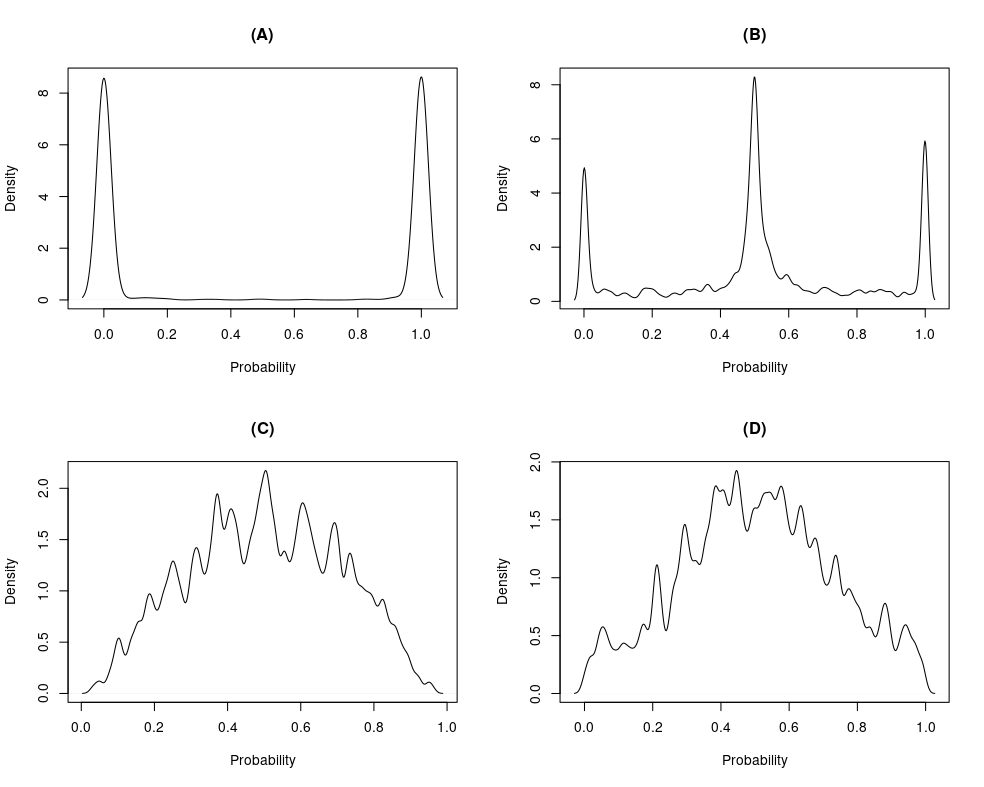
\includegraphics[width=1\textwidth]{prior_elicitation}
	\caption[Prior predictive simulation. Examples of uninformative and mildly informative priors.]%
	{Prior predictive simulation. Examples of uninformative and mildly informative priors. The panels show the density for the probability of a binary outcome under: (A) uninformative prior on equation (\ref{eq:prior_el1}) and mildly informative prior on equation (\ref{eq:prior_el3}); and (B) uninformative prior on equation (\ref{eq:prior_el2}) and mildly informative prior on equation (\ref{eq:prior_el4}). Uninformative (black continuous lines), and mildly informative (blue discontinuous lines).}
	\label{fig:prior_elicitation}
\end{figure}

In our case, as stated in section \ref{sub_sect:bads}, because priors can be considered a part of the model assumptions, they can be chosen, evaluated, and revised as any other component of the model \cite{McElreath_2020}. In that sense, we motivate the use of mildly informative priors though a simple illustration. Consider an example similar to one outlined by \citet{Seaman_et_al_2012} and \citet{McElreath_2020}, where a simple latent variable model is defined as follows:
%
\begin{equation} \label{eq:prior_el1}
	\begin{split}	
		\theta &\sim N(0, 100) \\
		\text{logit}(p) &= \theta
	\end{split}
\end{equation}

\noindent where $\theta$ denotes a latent dimension, and $p$ denotes the probability of a binary outcome, defined by the logit-link function. For pedagogical purposes, we did not declared the distribution of the response, as we wanted to assess what the prior implied for its expected value/probability.

Panel (A) from figure \ref{fig:prior_elicitation} shows that the uninformative prior in equation (\ref{eq:prior_el1}) forces an unintended assumption onto the expected value of the outcome (black continuous line). The model is now highly `skeptical' of probabilities that are not zero or one. This means that we are effectively using highly regularizing priors, but opposite on how they are supposed to be used, i.e. to avoid visiting non-likely parameter spaces.

The scenario gets equally bad with the presence of hyper-parameters, and even less extreme assumptions. Consider the following example:
%
\begin{equation} \label{eq:prior_el2}
	\begin{split}
		v &\sim \log N(0, 3) \\	
		\theta &\sim N(0, v) \\
		\text{logit}(p) &= \theta
	\end{split}
\end{equation}

\noindent where $v$ is distributed as a log-normal distribution ($v>0$). Panel (B) from figure \ref{fig:prior_elicitation} shows that the uninformative priors in equation (\ref{eq:prior_el2}) forces another unintended assumption on the expected value of the outcome (black solid line). The model is now highly `skeptical' of probabilities that are not $p = \{0, 0.5, 1\}$. Again is like using regularizing priors but ``in reverse".

Luckily, these extreme priors can be overcome with enough data. However, that does not discard the need to address the issue, as much of the time, researchers do not have a clear definition of how much is ``enough" data.

In that sense, mildly informative priors can help alleviate the concern. Mildly/weakly informative priors are prior distributions that are not supplying any controversial information, are consistent with the likelihood, and are strong enough to pull the data away from inappropriate inferences \cite{Gelman_et_al_2014}. To illustrate its use, consider a mildly informative prior on equation (\ref{eq:prior_el1}):
%
\begin{equation} \label{eq:prior_el3}
	\begin{split}	
		\theta &\sim N(0, 1) \\
		\text{logit}(p) &= \theta
	\end{split}
\end{equation}

Notice now $\theta$ has a prior that is consistent with common IRT applications, and its distribution does not force the expected value of the outcome to be as extreme, as in the uninformative case. Panel (A) from figure \ref{fig:prior_elicitation} shows the prior probability of the outcome can now be in the full $[0,1]$ range, where extreme probability values are assumed less likely (blue discontinuous line vs black solid line).

Similarly, in the presence of hyper-parameters we can set mildly informative priors in the following form:
%
\begin{equation} \label{eq:prior_el4}
	\begin{split}
		v &\sim \log N(0, 0.5) \\	
		\theta &\sim N(0, v) \\
		\text{logit}(p) &= \theta
	\end{split}
\end{equation}

\noindent where the blue discontinuous line on panel (B) of figure \ref{fig:prior_elicitation} shows its transformation into the expected value of the outcome.

One can imagine the procedure of prior elicitation will get more complicated with a larger number of parameter and hyper-parameters. Therefore, the use of prior predictive simulation will be a tool of high value for complex models, as in our current implementation. See section \ref{sub_sect:prior_pred_inv} for an example on the use of prior predictive investigation, under simulated data.



%%%%%%%%%%%%%%%%%%%%%%%%%%%%%%%%%%%%%%%%%%%%%%%%%%%%%%%%%%%%%%%%%%%%%%%
%%%%%%%%%%%%%%%%%%%%%%%%%%%%%%%%%%%%%%%%%%%%%%%%%%%%%%%%%%%%%%%%%%%%%%%

\section{To center or not to center} \label{sect:noncenter}

As pointed out by \citet{Betancourt_et_al_2013}, even the most simple hierarchical models present formidable pathologies, that no simple correction can be performed to visit the posterior distribution properly. This is true no matter the rotation/rescaling of the parameter, or the amount of data. 

A great example of this is what \citet{McElreath_2020} dubbed the Devil's funnel (depicted in figure \ref{fig:devil_CE_geom}), where the author shows that you do not need a complex model to start observing these issues. Consider the following joint distribution:
%
\begin{equation} \label{eq:devil}
	\begin{split}	
		v &\sim N(0, 3) \\
		\theta &\sim N(0, \text{exp}(v))
	\end{split}
\end{equation}

\noindent where $v$ is the \textit{hyper-parameter} of $\theta$, and $\theta$ is dependent on the samples of $v$. The latter is what the literature dubbed as the centered parametrization (CP).

This joint distribution might seem familiar, as bayesian hierarchical model practitioners often use it to ensure the standard deviation remains into the permitted parameter space ($\sigma \geq 0$). Similar types of requirements permeate IRT models. Moreover, it seems that any MCMC procedure would not have any issues exploring the joint distribution of these parameters, as they are normally distributed and there are only two of them, but we would be wrong. 

For pedagogical purposes, the example was run without data, as the author wanted to emphasize the pathologies are present even before we feed the data to our model. However, its easy to extrapolate that these issues will remain present when data is available. The reader can find the \texttt{stan} and \texttt{jags} implementations for these examples in Appendix \ref{appC1_1:noncenter}. The \texttt{stan} implementation replicates the example stated by \citet{Betancourt_et_al_2013} and \citet{McElreath_2020}.

Figure \ref{fig:devil_CE} show the chains resulting from implementing the model on equation (\ref{eq:devil}), through HMC (\texttt{stan}). As one can see from the figure, the joint posterior distribution is not explored properly. The chains show no sign of achieving ergodicity \cite{Metropolis_et_al_1953}, i.e. they do not show stationarity or convergence (top panels), nor a good mixing (middle and bottom panels). This is further supported by the \texttt{Rhat}, and effective sample sizes estimates \texttt{n\_eff} \cite{Gelman_et_al_2014}. The \texttt{Rhat} for all parameters did not properly approach the threshold of one (most of them were even above $1.05$), indicating the chains did not achieve convergence: the between-chain variability was larger than the within-chain variability. Furthermore, the effective samples sizes were $34$ and $293$ for $v$ and $\theta$, respectively; indicating the values of the chains remained highly correlated (see bottom panels). This is striking, as one expects effective sample sizes closer to the effective number of iterations ($3,000$, coming from $3$ chains with $1,000$ samples each, after warm-up).
%
\begin{figure}[h]
	\centering
	\begin{subfigure}
		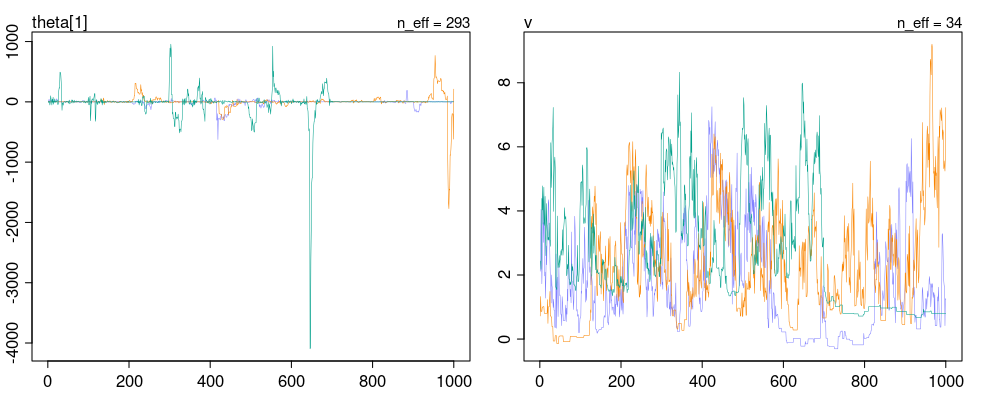
\includegraphics[width=.75\linewidth]{1_trace_CE_simple}
	\end{subfigure}
	%
	\begin{subfigure}
		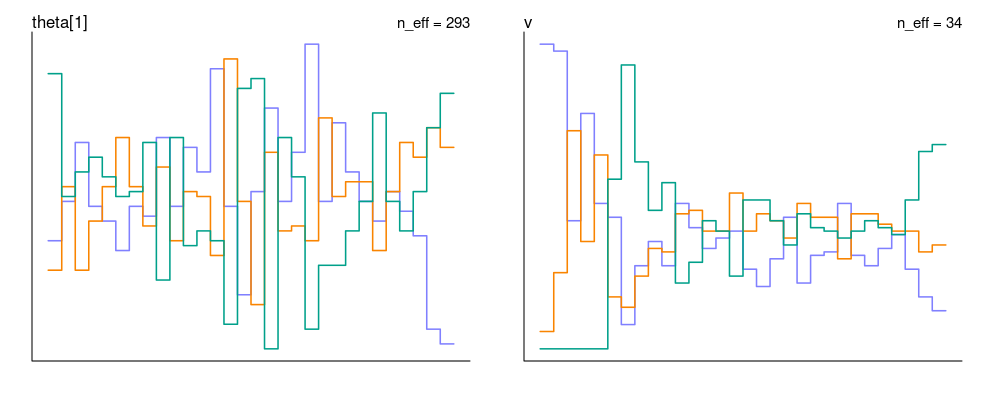
\includegraphics[width=.75\linewidth]{1_trank_CE_simple}
	\end{subfigure}
	%
	\begin{subfigure}
		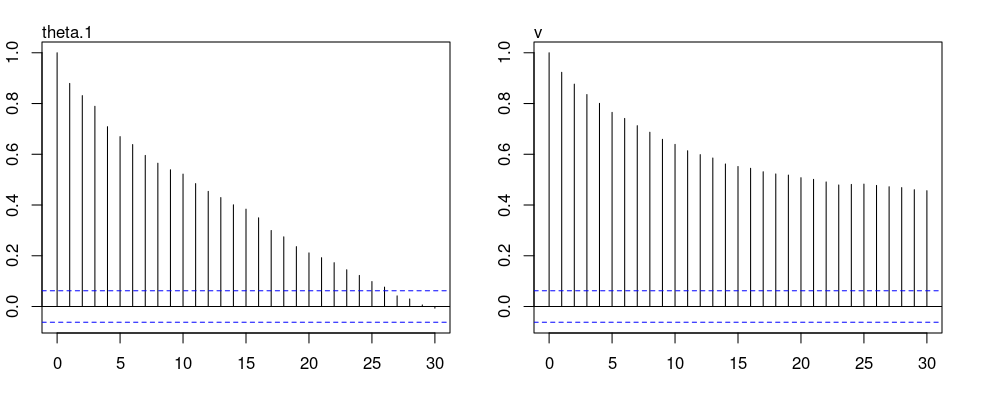
\includegraphics[width=.75\linewidth]{1_acf_CE_simple}
	\end{subfigure}
	%
	\caption[The Devil's funnel. Centered Parametrization. Stan.]%
	{The Devil's funnel. Centered Parametrization. (Top) Trace plots for the iterations on three chains. (Middle) Trank plots for the same data. (Bottom) Auto-correlation Functions (ACF) plot for the iterations.}
	\label{fig:devil_CE}
\end{figure}

%%%%%%%%%%%%%%%%%%%%%%%%%%%%%%%%%%%%%%%%%%%%%%%%%%%%%%%%%%%%%%%%%%%%%%%

\subsection{Wasn't HMC the solution to this?}

HMC is a powerful MCMC algorithm, and its benefits stand the test of other scenarios, as detailed by multiple authors \cite{McElreath_2020, Gelman_et_al_2014}. However, the issue with this example goes a little bit farther than what the algorithm can actually overcome, and this is true also for the Metropolis and Gibbs sampling algorithms. Nevertheless, we will see HMC still manages to be efficient within the constrains of the problem.
%
\begin{figure}[h]
	\centering
	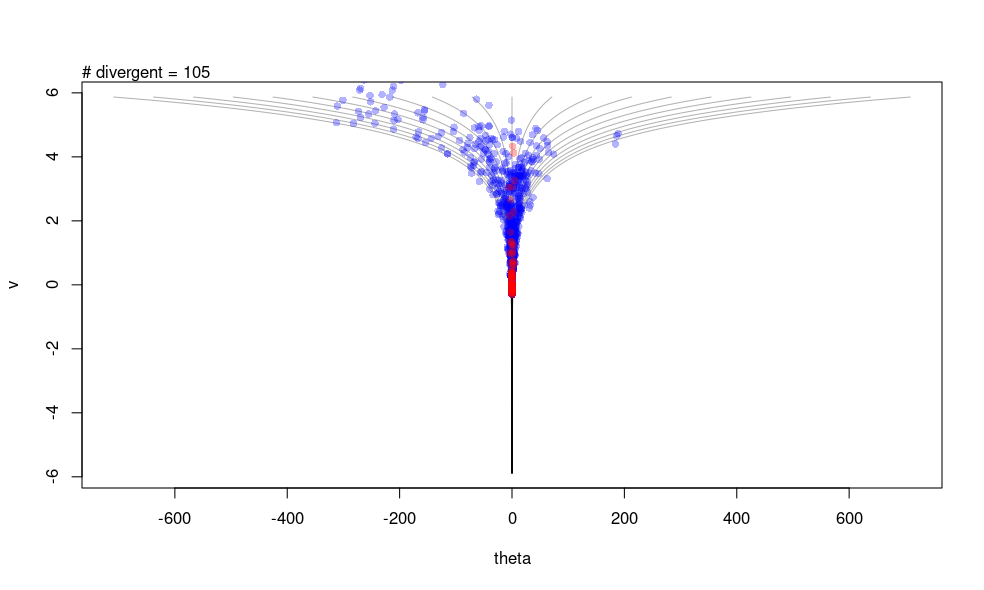
\includegraphics[width=1\linewidth]{1_funnel_CE_simple}
	%
	\caption[Posterior sampling geometry. Centered Parametrization.]%
	{Posterior sampling geometry. Centered Parametrization. (A) HMC exploration, blue points are accepted samples, red points denote divergent transitions. (B) Metropolis/Gibbs exploration, blue points are samples.}
	\label{fig:devil_CE_geom}
\end{figure}

Figure \ref{fig:devil_CE_geom} shows the posterior sampling geometry of the model in equation (\ref{eq:devil}), for the HMC algorithm (\texttt{stan}, left) and Metropolis/Gibbs sampler (\texttt{jags}, right), respectively. 

The first thing to notice is the complexity of the joint posterior geometry, with a steep funnel shape as the values of $v$ gets smaller and smaller. This makes sense, as the exponential of larger negative values, force the standard deviation of $\theta$ to be narrower and narrower around its mean (zero). 

The second thing to notice is that HMC (left panel) still manages to successfully explore the steep parameter space of $v$ and $\theta$. This can be observed through the blue points that are scattered in most of the geometry, albeit some parts are less visited (area where $\theta>0$). This does not happen under the Gibbs sampler. In fact, \texttt{jags} did not managed to escape the narrow funnel shape, no matter the number of iterations used in the adaptation, burn-in and sampling procedures\footnote{\texttt{stan} used $3$ chains with $1,000$ iterations for adaptation, and $1,000$ iterations for sampling. \texttt{jags} used $3$ chains with $5,000$ iterations for adaptation, $5,000$ iterations for burn-in, and $5,000$ iterations for sampling.} (panel B). Moreover, as shown in figure \ref{fig:devil_CE_simple_jags} (appendix), the traceplots indicate the chains are ``healthy", ignoring the clear lack of exploration of the joint distribution.

Finally, although HMC did not fully explore the joint distribution, at least the method let us know which parts of it did not manage to visit appropriately (see red points indicating divergent transitions). The last is important, because HMC gives us the opportunity to identify where can we improve our parametrization, something that is not available on Metropolis or Gibbs.


%%%%%%%%%%%%%%%%%%%%%%%%%%%%%%%%%%%%%%%%%%%%%%%%%%%%%%%%%%%%%%%%%%%%%%%

\subsection{So, how can we solve this?}

There are three proposed solutions for the previously explained issue: (i) adapt the HMC warm-up, (ii) use regularizing priors, and (iii) change the posterior sampling geometry. This section will explain briefly the first, outline the geometrical perspective of the second (as its results are well studied); and advocate for the benefits of the third, in the context of IRT models.

%%%%%%%%%%%%%%%%%%%%%%%%%%%%%%%%%%%%%%%%%%%%%%%%%%%%%%%%%%%%%%%%%%%%%%%

\subsubsection{Adapt warm-up}

As explained in previous sections, the HMC requires a warm-up phase to adapt the parameters' sampling. In it, two meta-parameters are ``tuned-in" (\texttt{leapfrogs} and \texttt{step size}); while a rejection criterion (\texttt{adapt\_delta}) remains constant. As we recall, HMC follows a rejection procedure that inform us when the method was not able to maintain the ``energy" of the system, producing a divergent transition; and in the core of this procedure is the rejection criterion.

As it is pointed out by \citet{McElreath_2020}, divergent transitions do not damage directly our posterior distribution approximation, but they do hurt indirectly, as the region where divergent transitions occur is hard to properly explore.

Therefore, to reduce the impact of the divergent transitions, the user can increase the criterion's threshold above the default values (\texttt{adapt\_delta}$=0.95$), resulting in slower but more confident exploration of the posterior distribution.

Finally, in regards to this solution, two important point should be kept in mind. First, the solution is method specific, as HMC is the only algorithm that uses this parameter. And second, the solution forces the method to make a slower posterior investigation, therefore requiring the user to set longer chains to achieve ergodicity.

%%%%%%%%%%%%%%%%%%%%%%%%%%%%%%%%%%%%%%%%%%%%%%%%%%%%%%%%%%%%%%%%%%%%%%%

\subsubsection{Regularizing priors} \label{subsub_sec:reg_prior}

As previously mentioned, several authors have shown the benefits of using weakly regularizing priors in diverse types of models \cite{McElreath_2020, Gelman_et_al_1996b, Jaynes_1985}. However, few of them have described how the use of regularizing priors work from a geometrical perspective. Consider the use of a regularizing prior on equation (\ref{eq:devil}):
%
\begin{equation} \label{eq:devil_prior}
	\begin{split}	
		v &\sim N(0, 1) \\
		\theta &\sim N(0, \text{exp}(v))
	\end{split}
\end{equation}
%
\begin{figure}[h]
	\centering
	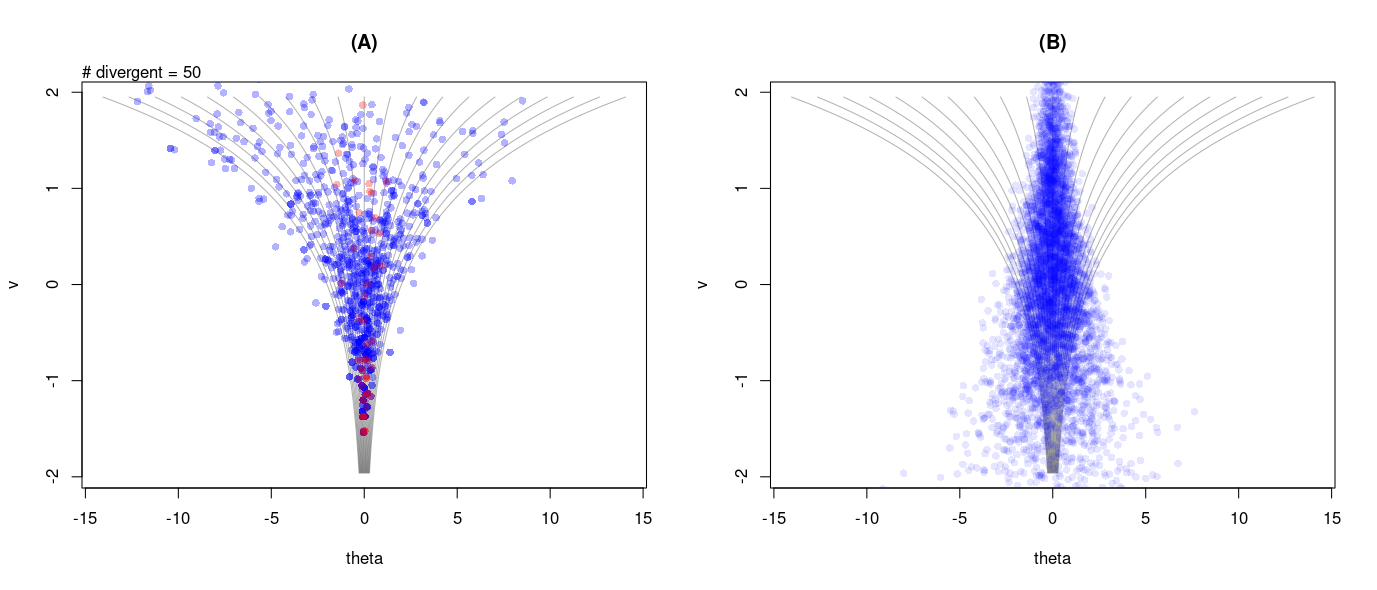
\includegraphics[width=1\linewidth]{2_funnel_CE_priors}
	%
	\caption[Posterior sampling geometry. Centered Parametrization with mildly informative priors.]%
	{Posterior sampling geometry. Centered Parametrization with mildly informative priors. (A) HMC exploration, blue points are accepted samples, red points denote divergent transitions. (B) Metropolis/Gibbs exploration, blue points are samples.}
	\label{fig:devil_prior_geom}
\end{figure}

Figure \ref{fig:devil_prior_geom} shows the joint posterior sampling geometry of equation (\ref{eq:devil_prior}), for the HMC algorithm (\texttt{stan}, left) and Metropolis/Gibbs sampler (\texttt{jags}, right), respectively. 

The first thing to notice from the figure is that the geometry available for exploration seems more broad. However, what is actually happening is that by adding information about $v$, we are ``zooming" into the posterior geometry observed in figure \ref{fig:devil_CE_geom}, according to the range of the new priors. This further benefits the exploration of the posterior, as extreme ranges don't have to be visited from the start, e.g. the narrow funnel in the range $[-6,-2]$ of $v$ from figure \ref{fig:devil_CE_geom}.

The second thing one can notice is that HMC does not ``loose time" exploring sections of the posterior distribution that are not needed. Surprisingly in contrast, the Gibbs sampler explore non-useful sections and leaves the useful ones unexplored. Again, this is true no matter the number of iterations used in the adaptation, burn-in and sampling procedures\footnote{the author used the same settings as in the previous example.}. Moreover, the chains in figure \ref{fig:devil_CE_prior_jags} (appendix) seem to be ergodic, ignoring the clear lack of exploration of the joint distribution, as in the previous example.

Third, we see that using regularizing priors reduced the number of \texttt{stan}'s divergent transitions from $150$ (in the previous example) to $50$. Although we still observe them in the steepest part of the geometry. Such information is not provided by \texttt{jags}.

Finally, we notice a mild improvement on the trace, tranks and ACF plots in figure \ref{fig:devil_prior}, compared to figure \ref{fig:devil_CE} in the previous example.
%
\begin{figure}[h] 
	\centering
	\begin{subfigure}
		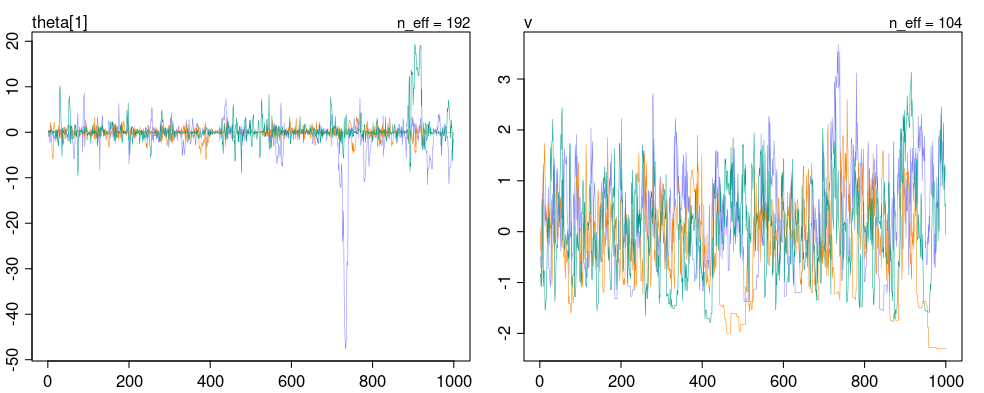
\includegraphics[width=.75\linewidth]{2_trace_CE_priors}
	\end{subfigure}
	%
	\begin{subfigure}
		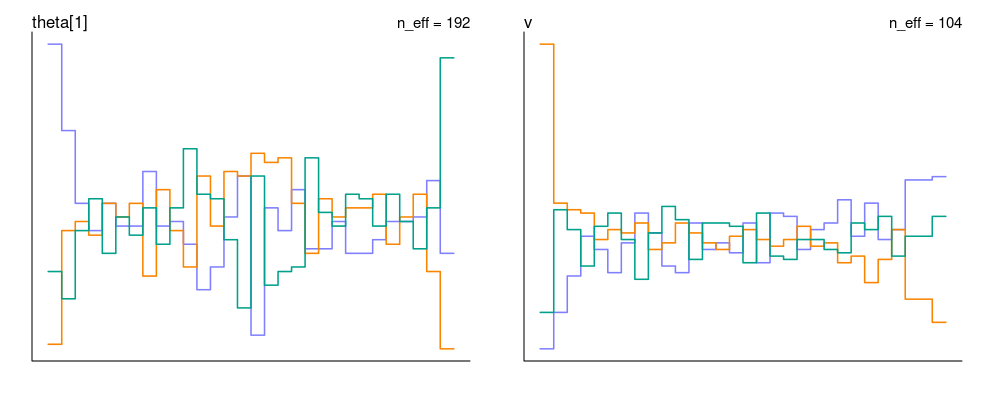
\includegraphics[width=.75\linewidth]{2_trank_CE_priors}
	\end{subfigure}
	%
	\begin{subfigure}
		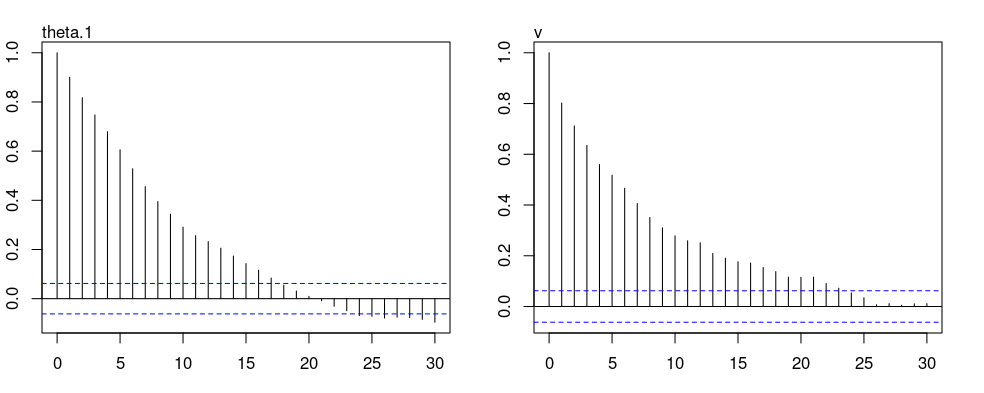
\includegraphics[width=.75\linewidth]{2_acf_CE_priors}
	\end{subfigure}
	%
	\caption[The Devil's funnel. Centered Parametrization with prior information.]%
	{The Devil's funnel. Centered Parametrization with mildly informative priors. (Top) Trace plots for the iterations on three chains. (Middle) Trank plots for the same data. (Bottom) Auto-correlation Functions (ACF) plot for the iterations.}
	\label{fig:devil_prior}
\end{figure}

%%%%%%%%%%%%%%%%%%%%%%%%%%%%%%%%%%%%%%%%%%%%%%%%%%%%%%%%%%%%%%%%%%%%%%%

\subsubsection{Non-centered parametrization} \label{subsub_sec:NCP}

It would seem that, increasing the regularizing power of the priors is the answer to get rid of the sampling issues raised by a complex posterior sampling geometry. However, there is a limit on the information a prior can contain, without imposing strong assumptions about the parameters (see section \ref{sub_sect:prior_pred} for an example). Furthermore, sometimes researchers want the information on the data dominates the posterior parameter space. In those cases, imposing even mildly informative priors is a solution that is out of the picture.
%
\begin{figure}[h]
	\centering
	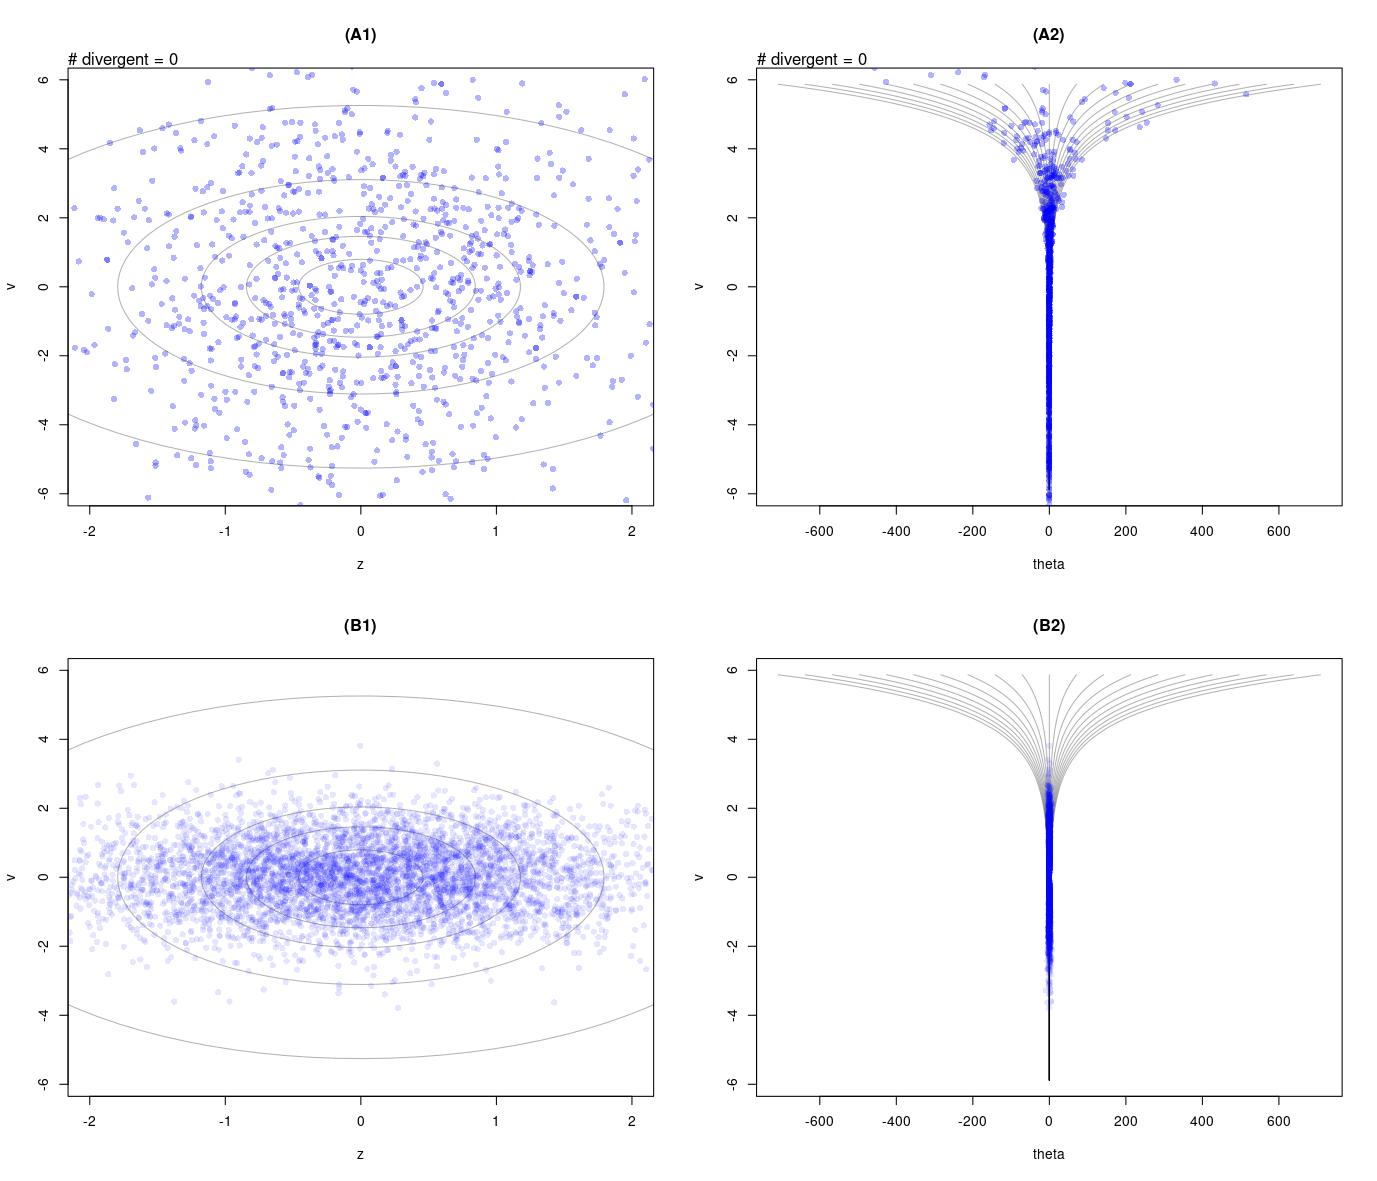
\includegraphics[width=1\linewidth]{3_funnel_NC}
	%
	\caption[Posterior sampling geometry. Non-Centered Parametrization.]%
	{Posterior sampling geometry. Non-Centered Parametrization. (A1, B1) geometry defined by the independent parameters $v$ and $z$. (A2, B2) Original sampling geometry defined by $v$ and $\theta$. (A1, A2) HMC algorithm (\texttt{stan}). (B1, B2) Metropolis/Gibbs sampler (\texttt{jags}). Blue points are accepted samples. Red points denote divergent transitions.}
	\label{fig:devil_NC_geom}
\end{figure}

In this context, \citet{Betancourt_et_al_2013} indicated that prior information can be included in the model, not only through the prior distributions, but also by encoding it in the model itself, taking advantage of the hierarchical structure explicitly, i.e. change the posterior sampling geometries. 
%
\begin{figure}[h]
	\centering
	\begin{subfigure}
		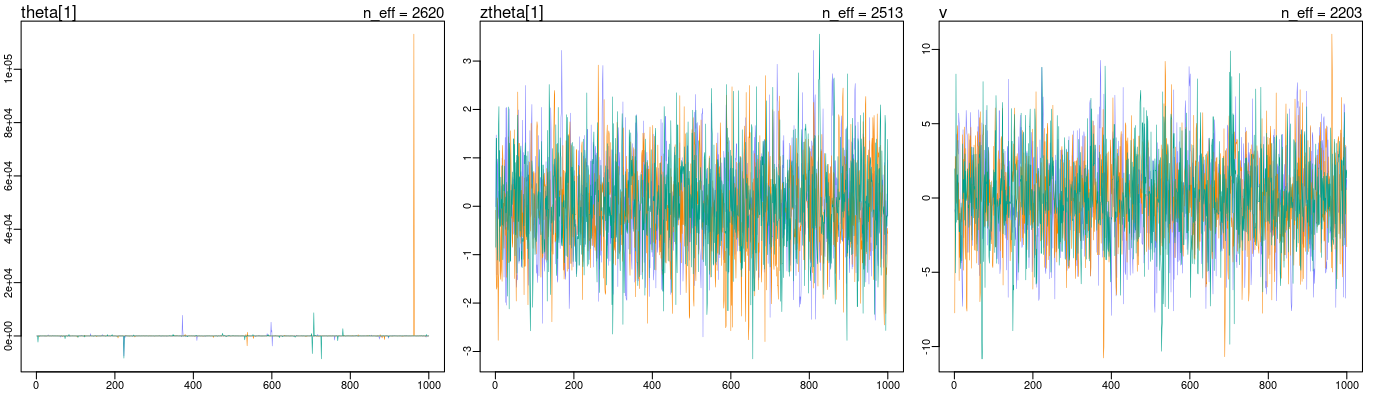
\includegraphics[width=1\linewidth]{3_trace_NC}
	\end{subfigure}
	%
	\begin{subfigure}
		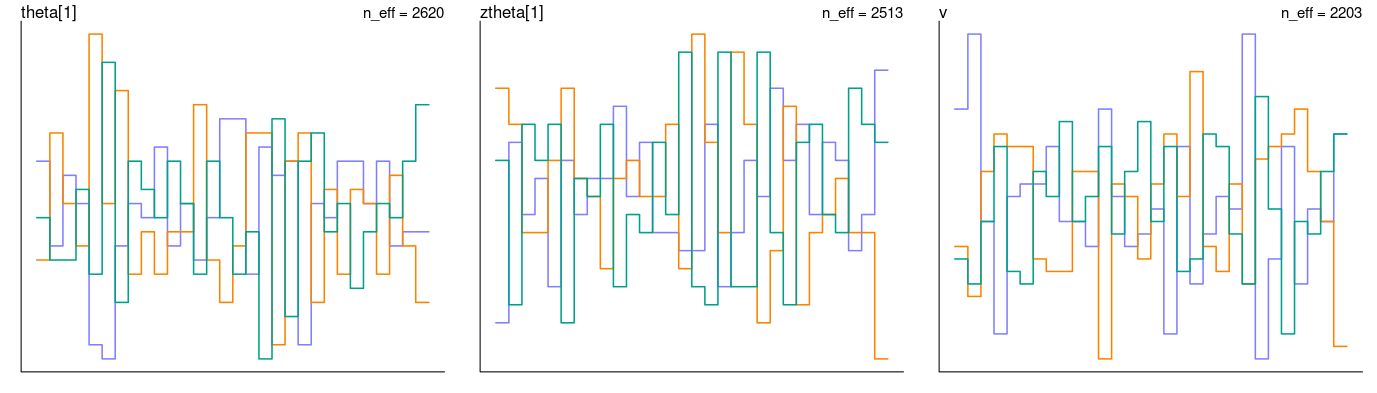
\includegraphics[width=1\linewidth]{3_trank_NC}
	\end{subfigure}
	%
	\begin{subfigure}
		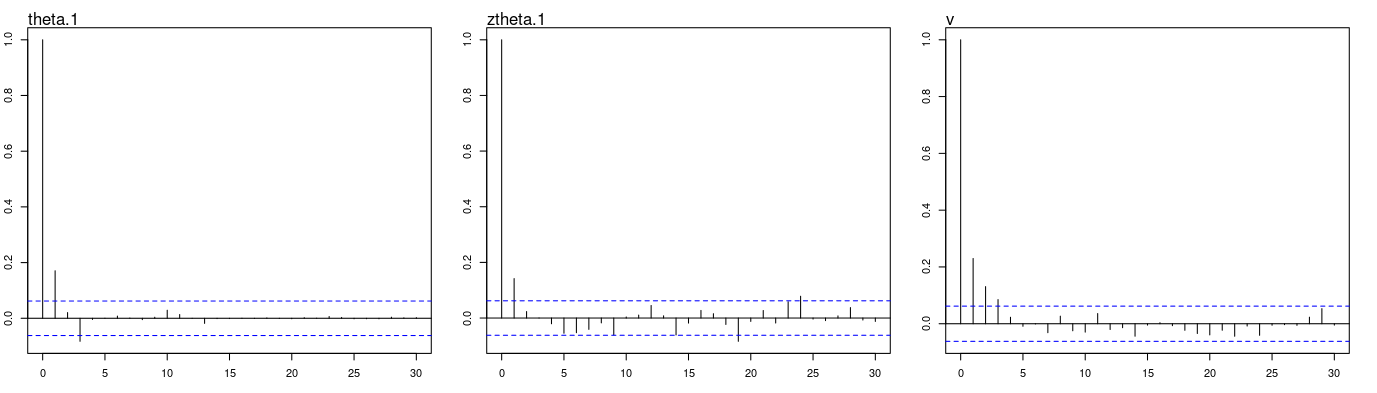
\includegraphics[width=1\linewidth]{3_acf_NC}
	\end{subfigure}
	%
	\caption[The Devil's funnel. Non-centered Parametrization.]%
	{The Devil's funnel. Non-centered Parametrization. (Top) Trace plots for the iterations on three chains. (Middle) Trank plots for the same data. (Bottom) Auto-correlation Functions (ACF) plots for the iterations.}
	\label{fig:devil_NC}
\end{figure}

Following \citet{Papaspiliopoulos_et_al_2003, Papaspiliopoulos_et_al_2007}, and \citet{Betancourt_et_al_2013}, under the Bayesian framework, a change in geometry consist on a model re-parameterization that seeks to remove the dependence of parameters on other sampled parameters, therefore favoring the performance of the MCMC chains. This is what the literature has dubbed as the non-centered parametrization (NCP).

In light of previous examples, changing the posterior sampling geometry means to modify equation (\ref{eq:devil}) in the following way:
%
\begin{equation} \label{eq:devil_NC}
	\begin{split}	
		v &\sim N(0, 3) \\
		z &\sim N(0, 1) \\
		\theta &= \text{exp}(v) \; z
	\end{split}
\end{equation}

\noindent notice $v$ has the original assumed variability, but now $\theta$ is defined in a way, that is no longer sample dependent on $v$, i.e. we no longer sample $\theta$ directly but $z$, and transform it back.

The motivation for this re-parametrization have seeds in the calculation of the standard score (z-sore). Notice that if $\theta \sim N(\mu_{\theta}, \sigma_{\theta})$ where $\sigma_{\theta} = \text{exp}(v)$, then $(\theta - \mu_{\theta})/\sigma_{\theta} = z$ and $z \sim N(0,1)$. Using this process in reverse, we notice $\theta = \mu_{\theta} + \sigma_{\theta} z = \text{exp}(v) \; z$ when $\mu_{\theta}=0$, then $\theta \sim N(0, \text{exp}(v))$. As the previous, there are transformation that can be done for other distributions, and they can even be extended to the multivariate normal case, through the use of the Cholesky decomposition \cite{McElreath_2020}.

Figure \ref{fig:devil_NC_geom} show the posterior sampling geometry for the HMC and Gibbs sampler, under the re-parametrization. Notice both algorithms manage to explore more successfully the posterior distribution, although the HMC does it a bit better on the extremes of $v$. Moreover, the HMC shows no divergent transitions, meaning the posterior is ``visited" without issues. Evidence of the latter can be as seen on figure \ref{fig:devil_NC}, where the chains show clear signs of stationarity, convergence and good mixing.

Finally, \citet{Papaspiliopoulos_et_al_2007} indicated that the success of the NCP strategy is largely dependent on the specifics of the model and data, i.e. neither CP or NCP is more ``optimal" than the other. The author pointed out that the natural CP showed better performance when conditional conjugacy was present, i.e. when the posterior distribution belonged to the same parametric family as the likelihood or prior distribution. On the other hand, the NCP worked as its complement, excelling when the previous requirement was not present. Therefore, due to this complementary behavior, it makes sense that recent advancements on the topic are focused on producing sample mechanisms located in a continuous between CP and NCP, as greater performance improvements can be obtained by leveraging on both, e.g. Interleaved HMC (iHMC) or Variational Inference (VI) \cite{Gelfand_et_al_1995, Gelfand_et_al_1996, Papaspiliopoulos_et_al_2003, Papaspiliopoulos_et_al_2007, Gorinova_et_al_2019}.

Chapter \ref{chap:simulation} and \ref{chap:application} will show the application of NCP in the context of an IRT model.
